% \documentclass[10pt, a4paper]{amsart}
\documentclass[%
reprint,
nofootinbib,
%superscriptaddress,
%groupedaddress,
%unsortedaddress,
%runinaddress,
%frontmatterverbose,
%preprint,
%showpacs,preprintnumbers,
%nofootinbib,
%nobibnotes,
%bibnotes,
amsmath,amssymb,
aps,
%pra,
%prb,
%rmp,
%prstab,
%prstper,
%floatfix,
]{revtex4-1}
\usepackage[]{graphicx}
\usepackage{float}
\usepackage[]{hyperref}
\usepackage[]{physics}
\usepackage[]{listings}
\usepackage[T1]{fontenc}
\usepackage{color}
\usepackage[]{subcaption}
\usepackage[ruled,vlined]{algorithm2e}
\usepackage{amssymb, amsmath}
\usepackage{caption}
\captionsetup{justification=raggedright,singlelinecheck=false}

\definecolor{mygreen}{rgb}{0,0.6,0}
\definecolor{mymauve}{rgb}{0.58,0,0.82}

\newcommand\todo[1]{\textcolor{red}{#1}}

\lstset{ %
	backgroundcolor=\color{white},   % choose the background color; you must add \usepackage{color} or \usepackage{xcolor}
	basicstyle=\footnotesize,        % the size of the fonts that are used for the code
	breakatwhitespace=false,         % sets if automatic breaks should only happen at whitespace
	breaklines=true,                 % sets automatic line breaking
	captionpos=b,                    % sets the caption-position to bottom
	commentstyle=\color{mygreen},    % comment style
	deletekeywords={...},            % if you want to delete keywords from the given language
	escapeinside={\%*}{*)},          % if you want to add LaTeX within your code
	extendedchars=true,              % lets you use non-ASCII characters; for 8-bits encodings only, does not work with UTF-8
	frame=single,	                   % adds a frame around the code
	keepspaces=true,                 % keeps spaces in text, useful for keeping indentation of code (possibly needs columns=flexible)
	keywordstyle=\color{blue},       % keyword style
	language=c++,                    % the language of the code
	otherkeywords={*,...},           % if you want to add more keywords to the set
	rulecolor=\color{black},         % if not set, the frame-color may be changed on line-breaks within not-black text (e.g. comments (green here))
	showspaces=false,                % show spaces everywhere adding particular underscores; it overrides 'showstringspaces'
	showstringspaces=false,          % underline spaces within strings only
	showtabs=false,                  % show tabs within strings adding particular underscores
	stepnumber=2,                    % the step between two line-numbers. If it's 1, each line will be numbered
	stringstyle=\color{mymauve},     % string literal style
	tabsize=2,	                     % sets default tabsize to 2 spaces
}


\begin{document}
	
\title{Monte Carlo simulations\\
	\normalsize{The Ising Model and Phase transition} \\
	\hrulefill\small{ FYS3150: Computational Physics }\hrulefill}

\author{Sigurd Sandvoll Sundberg}\homepage{https://github.com/SigurdSundberg/FYS3150}

\affiliation{%
	Department of Geosciences, University of Oslo\\
}%

\date{\today}

\begin{abstract}%1
In this article we have studied the 2-dimensional Ising model to study physical properties of ferromagnetic materials. We performed Monte Carlo simulation, with Metropolis sampling to with finite lattice sizes to reproduce the observed behavior of such materials. Starting at a small $2\times 2$ lattice to confirm the analytical results found by Lars Onsager\cite{LarsOnsager} in 1944, to expanding the code base and lattice size. Through this we studied the probability distribution function, equilibration time and acceptance ration. Finding that for a lattice of $20\times 20$, around $10^5$ Monte Carlo cycles are needed to reach the most likely state. Whilst the probability distribution function behaves as expected when we increase the temperature, allowing a large range of energies to be accessible. This is supported by the computed variance for the two temperatures studied, with the large of the two having a significantly larger variance. Lastly studied the phase transition and the critical temperature of the system, we gradually increased the lattice size with the use of parallelized and optimized code, achieve a significant speedup. From this we estimated the critical temperature found by Lars Onsager in the thermodynamic limit $T_c = 2.2692J/k_B$, which we found to be $T_c = 2.266J/k_B$ compared to the analytical value of . which can only be taken as a preliminary result as we have not account for the error in the interpolation used to achieve this value. 
\end{abstract}

\maketitle 

\section{Introduction} %1
The Ising model and its adaptions can be used to model a wide range of binary systems, from two party elections to magnetic behavior of magnets. It is normally used to describe the magnetic properties of ferromagnetic materials. It is a simplified classical model, where each spin is only allowed to interact with its nearest neighbors in a fixed lattice. Even though the Ising model is simple, many important physical quantities can be derived from it. Studying it numerically however has its problems. Even thought the system is binary, the number of different configurations of the lattice scales exponentially with the dimensionality of the lattice, this limits what properties we are able to calculate, for instance the probability distribution function is impossible to calculate. To solve this problem, Monte Carlo based Metropolis algorithm will be used. The Metropolis algorithm is a sampling algorithm that can be used to sample the probability distribution function of complicated systems. This enables us to sample the system and approximate with relative ease, accurately and being able to find the physical properties observed. We are able to test our results against the analytical results found by Lars Onsagr\cite{LarsOnsager}. 

In this article we will study a $2\times 2$ lattice, to bench mark our code against analytical results. Before moving onto  lattice size of $20\times 20$ and studying the equilibration time, probability distribution and acceptance ratio of spin-flips. Followed by studying how we can improve the run time of the Monte Carlo simulations, so we can tackle larger systems. For the larger systems up to $100 \times 100$ we will try to deduce the physical properties we expect the system to follow, such as phase transition. From this data we will also calculate the critical temperature by assuming a power law around the critical temperature, based on the data from the phase transition study. 

We will first cover the theory used, before tackling the algorithm and methods used to through the article to gather our results. Following we will present our results and discuss the findings and their implications, before concluding our work. 
\section{Theory} %1
The Ising model is a binary system, where the objects at each lattice site can take one of two values, either spin up or spin down. 
The energy of the Ising model, with no external magnetic field can be expressed as 
\begin{equation}
	E = -J\sum_{\langle k,e \rangle} s_ks_e,
\end{equation}
where we sum over the nearest neighbors interactions at each lattice site and $s_i$ can take the values $\pm 1$, which represents either spin up or spin down, respectively. 

We will in this article use natural units such as $k_B = J = 1$, where $k_B$ is the Boltzmann constant. 
\subsection{Canonical Ensemble} %1
In this article we will be working with an canonical ensemble, where the energy follows an expectation value at a given temperature. For us to calculate the expectation values such as the mean energy $\langle E \rangle$, we will be using a probability distribution, namely the Boltzmann distribution
\begin{equation}\label{eq:boltz}
	P_i(\beta) = \frac{e^{-\beta E_i}}{Z}
\end{equation}
where $\beta = 1/k_BT$ being the inverse temperature, $k_B$ is the Boltzmann constant, $E_i$ is the energy at microstate $i$ and Z is the partition function. We will in this article use natural units, that is $k_B = J = 1$. 

The partition function Z is given as 
\begin{equation}\label{eq:Z}
	Z = \sum_{i=1}^{M}e^{-\beta E_i},
\end{equation} 
where we sum over all microstates M.

The expectation value of the energy can be calculated from the probability distribution $P_i$ as 
\begin{equation}\label{eq:E}
	\langle E\rangle = \sum_{i=1}^{M}E_iP_i(\beta) = \frac{1}{Z}\sum_{i=1}^ME_ie^{-\beta E_i}
\end{equation}

The corresponding variance is defined as 
\begin{equation}
	\begin{split}
\sigma_E^2 &= \langle E^2 \rangle -\langle E\rangle^2 \\
&= \frac{1}{Z}\sum_{i=1}^ME_i^2e^{-\beta E_i} - \left(\frac{1}{Z}\sum_{i=1}^ME_i^2e^{-\beta E_i}\right)^2
	\end{split}
\end{equation}
If we divide by $k_BT^2$, we obtain the specific heat 
\begin{equation}\label{eq:cv}
	C_v = \frac{1}{k_BT^2}\left(\langle E^2 \rangle -\langle E\rangle^2\right).
\end{equation}

In the same way we can evaluate the mean magnetization through 
\begin{equation}\label{eq:M}
	\langle\mathcal{M}\rangle = \sum_i^M\mathcal{M}P_i(\beta) = \frac{1}{Z}\sum_i^M\mathcal{M}e^{-\beta E_i}
\end{equation}
and the corresponding variance 
\begin{equation}
\begin{split} 
		\sigma_\mathcal{M}^2			&=\langle \mathcal{M}^2 \rangle -\langle \mathcal{M}\rangle^2 \\
			&= \frac{1}{Z}\sum_{i=1}^M\mathcal{M}_i^2e^{-\beta E_i} - \left(\frac{1}{Z}\sum_{i=1}^M\mathcal{M}_i^2e^{-\beta E_i}\right)^2.
		\end{split} 
\end{equation}
This quantity defines the susceptibility $\mathcal{X}$
\begin{equation}\label{eq:x}
	\mathcal{X} = \frac{1}{k_BT}\left(\langle \mathcal{M}^2 \rangle -\langle \abs{\mathcal{M}}\rangle^2\right).
\end{equation}
\subsection{Phase Transition} %1
For our 2-dimensional Ising model, we from from a finite magnetization $\langle \mathcal{M} \rangle \neq 0$ to a paramagnetic phase with $\langle \mathcal{M} \rangle = 0$ at a critical temperature $T_C$. At this critical temperature the mean magnetization approaches zero with an infinite slope. Quantities like the heat capacity $C_v$ and the susceptibility $\mathcal{X}$ are discontinuous or diverge in the thermodynamic limit\cite{morten}, this happens as the lattice size L approaches infinity. As we can not simulate a infinite lattice, we will have to deal with approimating the critical temperature at which phase transition occurs. 

When studying a finite lattice, the variance in energy and magnetization no longer diverge or are discontinuous, however they scale as $\sim 1/\sqrt{M}$, where M is given as $M = 2^{L^2}$ microstates, for an $L\times L$ lattice. This means that we will not be able to observe a diverging behavior, but we will should be able to see as we increase the lattice size, that the peaks of $C_v$ and $\mathcal{X}$ should get sharper. 

The critical temperature for a finite lattice follows the following relation 
\begin{equation}\label{eq:3}
	T_C(L) = aL^{-1/\nu} + T_C(\infty),
\end{equation}
where $T_C(L)$ is the critical temperature found for a finite lattice size . From equation \eqref{eq:3} we will try to estimate $T_C(\infty)$ using $\nu = 1$ by studying the linear relation between the critical temperature and lattice size. 


\subsection{Analytical Results} %1
In 1944 Lars Onsager was the first to solve the Ising model analytically for a general lattice size L\cite{LarsOnsager}. He found that the critical temperature of the system is 
\begin{equation}
	T_C = \frac{2J}{k_Bln(1+\sqrt{2})}\simeq 2.269\dots
\end{equation} 
We will use the ideas from phase transition to try to estimate $T_C$, using larger lattice size. 

However first we need a benchmark for our code, where we will use a $2\times 2$ system with periodic boundary conditions to calculate numerical expectation values. The analytical expectation values and the partition function can be calculated through equations (\ref{eq:Z},\ref{eq:E}, \ref{eq:M}), and the value displayed in \autoref{tab:2x2}. Likewise we can find values of $E^2$ and $M^2$. 

We find that 
\begin{align}
	Z &= 12 + 4\cosh(8J\beta) && \beta = (k_BT)^{-1}\\
	\langle E\rangle &= -\frac{32J}{Z}\sinh(8J\beta)\\
	\langle E^2\rangle &= \frac{256}{Z}\cosh(8J\beta)\\
	\langle M\rangle &= 0\\
	\langle M^2\rangle &=\frac{32}{Z}\left(e^{8J\beta} + 1\right)\\
	\langle \abs{M}\rangle &= \frac{8}{Z}\left(e^{8J\beta} + 2\right)
\end{align}

From equation \eqref{eq:cv}, the heat capacity of the system is 
\begin{equation}
	C_v = \frac{256}{Zk_BT^2}\left( \cosh(8J\beta) - \frac{4}{Z}\sinh^2(8J\beta)\right)
\end{equation}
and we can find the susceptibility from equation \eqref{eq:x}, which can be expressed as 
\begin{equation}
	\mathcal{X} = \frac{32\beta}{Z}\left(e^{8J\beta} +1\right).
\end{equation}
\begin{table}
	\vspace{10pt}
	\caption{Display over the possible spin configurations for the $2\times 2$ lattice. As well as listing the energy and magnetization of system.}
	\label{tab:2x2}
\begin{tabular}{|c|c|c|c|c|}
	\hline 
	$N_\uparrow$ & Degeneracy & E  & M & Configurations\\
	\hline
	4 & 1 & -8J & 4 & $\begin{bmatrix}\uparrow & \uparrow \\ \uparrow&\uparrow\end{bmatrix}$\\
	3 & 4 & 0 & 2 & $\begin{bmatrix}\downarrow & \uparrow \\ \uparrow&\uparrow\end{bmatrix}\begin{bmatrix}\uparrow & \downarrow \\ \uparrow&\uparrow\end{bmatrix}\begin{bmatrix}\uparrow & \uparrow \\ \downarrow&\uparrow\end{bmatrix}\begin{bmatrix}\uparrow & \uparrow \\ \uparrow&\downarrow\end{bmatrix}$\\
	2 & 4 & 0 & 0 &$\begin{bmatrix}\downarrow & \downarrow \\ \uparrow&\uparrow\end{bmatrix}\begin{bmatrix}\uparrow & \uparrow \\ \downarrow&\downarrow\end{bmatrix}\begin{bmatrix}\downarrow & \uparrow \\ \downarrow&\uparrow\end{bmatrix}\begin{bmatrix}\uparrow & \downarrow \\ \uparrow&\downarrow\end{bmatrix}$\\
	2 & 2 & 8J & 0&$\begin{bmatrix}\downarrow & \uparrow \\ \uparrow&\downarrow\end{bmatrix}\begin{bmatrix}\uparrow & \downarrow \\ \downarrow&\uparrow\end{bmatrix}$\\
	1 & 4 & 0 & -2&$\begin{bmatrix}\uparrow & \downarrow \\ \downarrow&\downarrow\end{bmatrix}\begin{bmatrix}\downarrow & \uparrow \\ \downarrow&\downarrow\end{bmatrix}\begin{bmatrix}\downarrow & \downarrow \\ \uparrow&\downarrow\end{bmatrix}\begin{bmatrix}\downarrow & \downarrow \\ \downarrow&\uparrow\end{bmatrix}$\\
	0 & 1 & -8J & -4&$\begin{bmatrix}\downarrow & \downarrow \\ \downarrow&\downarrow\end{bmatrix}$\\
	\hline
\end{tabular}
\end{table}


\section{Algorithms}%1
We will be studying the 2-dimensional Ising model, through the use of Monte Carlo methods. Monte Carlo methods are class of computational algorithms, which use repeated random sampling to obtain numerical solutions. The can stretch from easy and trivial to implement to more advanced models where one utilizes different properties of a system to create more efficient algorithms. 

Random sampling with Monte Carlo method gives an asymptotic approximation error of $\sigma/\sqrt{N}$. Where $\sigma$ is the variance of the system and $N$ is the number of samples\cite{morten}. Compared to simpler methods for approximating numerical results, the Monte Carlo method performs poorly when the sample size is small. Thus it could be infeasible for simpler problems to apply Monte Carlo methods to simple systems. However the Ising model has not a simple system to simulate and fits the Monte Carlo method perfectly. 
\subsection{Markov Chains}%1
A Markov process (or chain) generates random states by use of random walks, that depends on a chosen probability distribution. A move from state $i$ to a new state $j$ can be described by a \textit{transition probability} $P(i\rightarrow j)$, which is the probability that the system will go from state $i$ to state $j$. 

If we let a Markov chain run for long enough under certain conditions, the system will reach its most likely state, regardless of initial state. In our case the most likely state is the equilibrium state of the system, with the probability distribution $w_j(t_k) = e^{\beta E_j}$. The time development of our probability distribution is given by 
\begin{equation}
	w_{j}(t_{k+1}) = P(i \rightarrow j)w_i(t_k) = P_{ij}w_i(t_k).
\end{equation}
In vector-matrix representation, we have 
\begin{equation}
	\vec{w}(t_{k+1}) = \mathbf{P}\vec{w}(t_k)
\end{equation}
where the transition probability $P_{ij}$ is represented on matrix form. 
The system is said to be in its most likely state when $\abs{\abs{w(t_{k+1}) - w(t_k)}} \rightarrow 0$. 

Following are some properties that the Markov process must obey. 
\subsubsection{Time Independence}%1
The transition probability must be time-independent, such that for a given time $t_v$, the probability for transitioning from a state $i \rightarrow j$ is the same as at time $t_u$.

The second part of the time independence is that $P(i \rightarrow j)$ should only be dependent on the states $i$ and $j$, that is the system is said to be "without history", independent of the time evolution of the system. 
\subsubsection{State Change}%1
A Markov chain must put the system in some state $j$ given a state $i$. So the system follows the following equation 
\begin{equation}
	\sum_j P(i\rightarrow j) = 1,
\end{equation}
this includes a state change from $i \rightarrow i$, such that $P(i \rightarrow i) \neq 0$.
\subsubsection{Ergodicity}%1
A last principle for the Markov chain is that:  
\textit{It is possible to reach any state $j$, from any state $i$ given a long enough Markov chain}. This condition is  called ergodicity. It is important because every state $i$ in the Boltzmann distribution has a non-zero probability. 
\subsection{Metropolis Algorithm}%1
In most cases, including ours the transition probability $P_{ij} = P(i\rightarrow j)$ is not known.  A Markov chain is such a process where the transition probability is generally unknown. This is where the Metropolis algorithm comes to the rescue. 

We can model the transition probability as the product of two probabilities. One probability of accepting the proposed move from state $i$ to state $j$ and the other probability for making the transition to the state $j$ being in the state $i$\cite{morten}. We will label these probabilities as $A(i \rightarrow j)$ and $T(i \rightarrow j)$, respectively. Our transition probability then reads 
\begin{equation}
	P(i \rightarrow j) = T(i \rightarrow j)A(i \rightarrow j).
\end{equation}
We want to derive the probabilities $A$ and $T$, such that $w_j(t_{k+1}) = w_j{t_k}$ when $t\rightarrow\infty$, starting from any initial distribution. 

As we are modeling our system as a Markov chain, we require that as as $t\rightarrow\infty$ we have 
\begin{align}
	\sum_i w_iT(i \rightarrow j)A(i \rightarrow j) &=\sum_i w_iT(j \rightarrow i)A(j \rightarrow i)\\
	&= 	\sum_i w_iP(j \rightarrow i)
\end{align}
using that $\sum_i P(j\rightarrow i) = 1$, we have 
\begin{equation}
	w_j = \sum_i w_iT(i\rightarrow j)A(i\rightarrow j) = \sum_i w_iP(i\rightarrow j)
\end{equation}
which is the standard Markov chain equation when a steady state has been reached. 

\subsubsection{Detailed Balance} %1
In general the condition that the probabilities should be equal, is normally not enough to ensure we reach the most likely state. We could end up in a cyclic solution where we go back and forth between to solutions. To counter this we will introduce detailed balance\cite{LarsOnsagerIrreversible}
\begin{equation}
	P(i\rightarrow j)w_i = P(j\rightarrow i)w_j.
\end{equation}

At equilibrium detailed balance gives us 
\begin{equation}
	\frac{P(i\rightarrow j)}{P(j\rightarrow i)} = \frac{w_j}{w_i},
\end{equation}
rewriting in terms of T and A we have 
\begin{equation}\label{eq:detailed balance}
	\frac{T(i\rightarrow j)A(i\rightarrow j)}{T(j\rightarrow i)A(j\rightarrow i)} = \frac{w_j}{w_i}.
\end{equation}
This condition ensures that it is our probability distribution that is reach when the system reaches equilibrium\cite{morten}.

With our probability distribution given by the Boltzmann distribution \eqref{eq:boltz}, the partition function \eqref{eq:Z} is infeasible to calculate and brute force Monte Carlo calculation will not results in the microstates which are important at equilibrium. To select the contributions that are important to the equilibrium, we need to use the detailed balance which is just given by a ration of probabilities. This makes us able to never have to calculate the partition function $Z$. 
For Boltzmann distribution the detailed balance results in 
\begin{equation}\label{eq:boltzmann relation}
	\frac{w_j}{w_i} = e^{-\beta \left(E_j - E_i\right)}.
\end{equation}

For the Ising model, a change in state from $i \rightarrow j$, would mean one of two things. Either a spin-flip or no change at all. This selection of states has to results in the Boltzmann distribution otherwise, our choice of microstates is wrong. Leading to us getting wrong results when sampling the system. 

\subsubsection{The Metropolis Algorithm Specialized}%1
The simplest form of the Metropolis algorithm is assuming that the transition probability $T(i\rightarrow j)$ is symmetric, implying that $T(i\rightarrow j) = T(j\rightarrow i)$. Using this we have from equation \eqref{eq:detailed balance} and equation \eqref{eq:boltzmann relation}
\begin{equation}
	\frac{A(i\rightarrow j)}{A(j\rightarrow i)} = e^{-\beta \left(E_j - E_i\right)}.
\end{equation}

Suppose $E_j > E_i$. Since it is only the ration that needs to obey the equality, we can make the algorithm more efficient by setting the largest of the two acceptance ratios to 1. 
Then we have 
\begin{equation}
		\frac{A(i\rightarrow j)}{A(j\rightarrow i)} = e^{-\beta \left(E_j - E_i\right)} < 1,
\end{equation}
where we impose $A(j\rightarrow i) = 1$. When $E_j < E_i$, the energy of the system is lowered and we accept the state change regardless. The acceptance probability can be summarized as 
\begin{equation}
	A(i \rightarrow j) = 
	\left\lbrace
	\begin{split}
		&e^{-\beta \left(E_j - E_i\right)},  && E_j - E_i > 0\\
		&1, && else.
	\end{split}
	\right.
\end{equation} 
Or in a different way, we can write the following \texttt{if($\Delta$E < 0 or r<$e^{-\beta \left(E_j - E_i\right)}$) $\lbrace$We accept the proposed swap$\rbrace$}. This ensures that we will reach the most likely state, but allowing energy states are less likely to be accepted. Making the acceptance ratio, able to follow the principle of ergodicity. This is done by choosing a random number \texttt{r} from a uniform distribution between 0 and 1.

\subsection{Monte Carlo - Metropolis Algorithm}%1
If we combine the above principles our final algorithm for performing the Monte Carlo simulations can read as follows
\begin{algorithm}[H]\label{algo:metropolis}
	\SetAlgoLined
	\caption{Monte Carlo simulation with Metropolis sampling}
	\texttt{Pick T and $L_i$}	\\
	\texttt{Compute $E_i$ and $M_i$}\\
	\For{\texttt{i = 0; i < MC cycles; i++}}{
		\For{\texttt{j = 0; j < Total Spins; j++}}{
			\texttt{Sample a random index of the spin matrix}\\
			\texttt{Compute $\Delta E$}\\
			\If{\texttt{$\Delta E$ < 0 or r < $e^{-\beta\Delta E}$}}{
				\texttt{Accept the flip}\\
				\texttt{Update E and M}\\
			}
			\texttt{Update the mean values for E and M}
		}
	}
	\texttt{Normalize all computed values}
\end{algorithm}
\section{Methods} %1
\subsection{Lattice Representation} %1
In order for us to represent the lattice in a efficient way, we will be using a matrix representation of the lattice. This enables us to easily apply our boundary conditions as well as enables us to with ease to increase the efficiency of our code by improving upon our algorithm. Both of which we will discuss shortly. 
\subsection{Periodic Boundary Conditions} %1
For boundary conditions we have chosen to use periodic boundary conditions, and as the lattice grows towards the thermodynamic limit, the choice of boundary conditions does not play a role. As approximating infinity with one additional element does not change the outcome. We are essentially going to approximate a large system, by making it slightly larger. 

When applying periodic boundary conditions we need a way to index ghosts points, that is indexing points outside the scope of our lattice representation. The simple way of doing so would be to implement \texttt{if}-statements to check whether we are indexing a ghost point or not. This is however slow and hard to optimize. 

A second possibility for handling the ghost points would be to expand our matrix to a $(L+2)\times(L+2)$ matrix, where we have the ability to index the ghosts points directly without the use of \texttt{if}-statements. However this runs into its own limitations, namely we would need to update the ghosts points whenever we change its corresponding value. In a 1-dimensional case this would lead to us having to update index 0 if we made a change to index n, for an array from 0 to n+1. This can be implemented using either \texttt{if}-statements or using properties of modulus operator. 

A third method, which is the one used in this project, is using the modulus operator directly on a $L\times L$ matrix. This is done by looking at the point of interest in the matrix and compute its neighboring indexes by the following equation
\begin{equation}
	\text{neighbor} = (\text{current} + \text{L} + \text{position}) \text{MOD} (\text{L})
\end{equation}
where current is the current matrix index, L is the dimensionality of the matrix and position is the index of the neighbor relative to current position. 
This equation handles both the ghost points and the normal points of the matrix and creates an efficient way for us to access all points of the matrix. 

By implementing this as an inline function, we are able to, at compile time, to reduce the time used of our program. 

\subsection{Exponential}  %1
In algorithm \ref{algo:metropolis} we are required to calculate $e^{-\beta\Delta E}$ for every spin, that is if we let M = number of Monte Carlo cycles and $L^2$ denote total number of spins, we would have to calculate this value $M\cdot L^2$ times. This would become exponentially large as we tackle larger lattice sizes with large amount of Monte Carlo cycles. To help us having to calculate the exponential millions of times per run, we can use some properties of the 2-dimensional lattice. 

One method of finding the change in energy after a lattice sweep is, sweeping through the lattice and calculate the energy. This is however not inefficient and not the chosen method. Instead we sweep through the lattice and only look at one spin at a time and updating the energy each time. This allows us to precalculate the values of the exponential as the change in energy at each lattice site only can take one of five values as shown in \autoref{tab:exp}. This enables ut for a given temperature T, to calculate all the possible values from the exponential prior to performing the Monte Carlo Metropolis algorithm. 

\begin{table}
	\vspace{10pt}
	\caption{The possible changes in energy $\Delta$E for the possible different neighbor configurations. We see that each lattice site only can have five different values for $\Delta$E, as they are only interacting with their nearest neighbors. The position of the neighboring spins does not change the change in energy, this is easy to show.}
		\label{tab:exp}
	\begin{tabular}{@{}|c|c|c|c|c|@{}}
		\hline
		Initial state & Final state & Initial E[J] & Final E[J] & $\Delta$E[J]\\\hline
$\begin{matrix}& \uparrow & \\ \uparrow & \uparrow & \uparrow \\ & \uparrow & \\ & & & \end{matrix}$         & $\begin{matrix}& \uparrow & \\ \uparrow & \downarrow & \uparrow \\ & \uparrow & \\ & & & \end{matrix}$ & -4 & 4 &     8                  \\
$\begin{matrix}& \downarrow & \\ \uparrow & \uparrow & \uparrow \\ & \uparrow & \\ & & & \end{matrix}$       & $\begin{matrix}& \downarrow & \\ \uparrow & \downarrow & \uparrow \\ & \uparrow & \\ & & & \end{matrix}$ & -2 &  2    & 4                  \\
$\begin{matrix}& \downarrow & \\ \downarrow & \uparrow & \uparrow \\ & \uparrow & \\ & & & \end{matrix}$     & $\begin{matrix}& \downarrow & \\ \downarrow & \downarrow & \uparrow \\ & \uparrow & \\ & & & \end{matrix}$ & 0 & 0   & 0                  \\
$\begin{matrix}& \downarrow & \\ \downarrow & \uparrow & \downarrow \\ & \uparrow & \\ & & & \end{matrix}$   & $\begin{matrix}& \downarrow & \\ \downarrow & \downarrow & \downarrow \\ & \uparrow & \\ & & & \end{matrix}$ & 2& -2  & -4                 \\
$\begin{matrix}& \downarrow & \\ \downarrow & \uparrow & \downarrow \\ & \downarrow & \\ & & & \end{matrix}$ & $\begin{matrix}& \downarrow & \\ \downarrow & \downarrow & \downarrow \\ & \downarrow & \\ & & & \end{matrix}$ & 4 & -4 & -8                 \\ \hline
	\end{tabular}

\end{table}

\subsection{Change in Energy and Magnetization}%1
As we are sweeping through our lattice we need to calculate the change in energy $\Delta$E and change in magnetization $\Delta$ M, for each flip we accept. As we saw from \autoref{tab:exp} the change in energy can only take one out of five values, since each spin site is only dependent on its four neighbors, as the other spins remain unchanged. Such that the change in energy $\Delta$E can be found the following way 
\begin{equation}
	\Delta E = E^j - E^i
\end{equation}
where $E^j$ denotes the energy after the flip and $E^i$ before the flip. We then have 
\begin{align}
	\Delta E &= -J\sum_{\langle k,e \rangle} s_k^js_e^j + J\sum_{\langle k,e \rangle} s_k^is_e^i\\
	&= -J\sum_{\langle k,e \rangle} s_k^j\left(s_e^j - s_e^i\right).
\end{align}
We can simplify this further, by looking at $s_e^i = 1$, if we flip it then $s_e^j = -1$ This means that $s_e^j-s_e^i = -2$. Also if $s_e^i = -1$ then $s_e^j = 1$, thus $s_e^j-s_e^i = 2$. Therefore $\Delta$E can be calculated using 
\begin{equation}
	\Delta E = 2Js_e^i\sum_{\langle k \rangle}s_k^i
\end{equation}

The change in magnetization is given in the same way. 
\begin{align}
	\Delta M &= M^j - M^i\\
	&= \sum_{k}s_k^j - \sum_{e}s_e^i\\
	&= s_k^j - s_k^i \\
	&= 2s_k^j
\end{align}


\subsection{Initial State}
To start of our representation of the lattice has no orientation. We would need to give it a starting orientation before performing the Monte Carlo simulations. We have two different ways of initializing the lattice. First, we can have all the spins point the same way, this gives a highly ordered lattice initially. 

A second option is to use a random number generator to randomly assign whether a spin points upwards or downwards, independent of neighboring spins. This gives us a configuration of high disorder. 

For small lattices this is computationally inexpensive, but as the lattice size grows initializing the lattice takes up more and more CPU cycles, if we need to initialize the lattice for each temperature. To reduce the number of CPU cycles we will look into how we can utilize small time steps and the equilibration time of the system to improve our calculations. 

\subsection{Equilibration Time} %1
At the start of each run, we have a lattice which is given one of two configurations. Either all spins pointing in the same direction, or all spins initial direction randomly chosen. This state is generally far away from the most likely state for a given temperature. As we are mainly interested in the expectation values of the system after reaching most likely state, we need to make sure that our system is at the most likely state before we start gathering data. 
There are different ways of determining when a system reaches its most likely state. 

One method is to choose a lattice size and run the Monte Carlo simulations, gathering all data and study the data afterwards. By looking at the expectation values as a function of the Monte Carlo cycles, we can approximate how long the system needs to run before reach the most likely state. Afterwards we can let the system run for the number of cycles we found before calculating the expectation values, this is a simple solution, and has its downsides. A downside is that the number of cycles needed to reach the most likely state, may depend on the initial condition and the temperature at the point of calculation. Therefore we can not be sure we have reached the most likely state before sampling our system for expectation values. To counter this we can overestimate the number of cycles we need, but that defeats the purpose of this method. 

A similar method which is easier to implement and does not require trial runs to find the approximation to the most likely state, is to simply slice away a portion of cycles and call it there. For low number of cycles, this also may not lead to the most likely state when we start to collect expectation values, however as the Monte Carlo method is greedy, we would normally use a number of cycles high enough to counter this problem outright. This is the standard approach for Monte Carlo methods and it is general practice to discard 10$\%$ to 15$\%$ of the runs before sampling the system, when it comes to the Ising model. As said however this does not guarantee that we are at an equilibrium position for the, as it depends on both the temperature and initial configuration. 

Another way we could use the fact that for a system in equilibrium, will have little change in the energy between two different configurations. Such that we can sample and check a few cycles for whether the change in energy and magnetization is sufficiently small, however defining sufficiently small is hard. And as we are dealing with random number generators we can never be sure that the consecutive runs are actually at an equilibrium state. So this would either never reach equilibrium or use a large amount of CPU cycles to find equilibrium. 

Lastly we can find the equilibrium from one time step to the next, with time step sufficiently small, by assuming that the equilibrium state for two lattices a small time step apart are the same. 

In this project we have applied a mixture of the different methods. We will be discarding 10$\%$ of the Monte Carlo cycles after the initialization of the lattice, to make sure we are hopefully close to the equilibrium, and start sampling for expectation values for a given T. After we are done sampling for a T, we will assume that the lattice is at equilibrium for the next temperature, with us having a sufficiently small time step. That is us using the old configuration to approximate the new configuration without having to equilibrate the lattice once more. For this we will use a time step between $0.05J/k_B$ to $0.01J/k_B$, depending on lattice size. 

\subsection{Optimization}%1
For the Monte Carlo methods, \texttt{c++} has been used as a programming language, and without any modifications, the language does not use multi-core processes. Meaning that we are running our programs on one core instead of utilizing the entire machine. As we are dealing with systems which requires many, many CPU cycles, we will use Message Parsing Interface(MPI), to parallelize the program. This allows us to perform multiple Monte Carlo simulations at a time, instead of one. We have here chosen to have each core, perform its own Monte Carlo simulation, effectively increasing the number of cycles we can perform for a given system. All the systems will be initialized by their own core and have no contact until all calculations are done. As an example, instead of running $10^6$ cycles on one core, we are able to run $4\cdot 10^6$ cycles, which is positive for the Monte Carlo method, as it is greedy. 

Another choice could have been to split the cycles into smaller chunks and have each core process a part of the total number of cycles. This is less expensive in CPU time, but in turn results in fewer samplings of the system.  

For this article all results with lattice sizes larger than $20\times20$, a parallelized version of algorithm \ref{algo:metropolis} has been used, and ran on a computer with 8 1GHz cores. 
\section{Results}% 1
\subsection{$2\times 2$ Lattice} %1
\autoref{tab:tableunordered} and \autoref{tab:tableordered} presents selected expectations values compared to the analytical values found earlier for a $2\times 2$ lattice at \texttt{}temperature T = 1.0. The expectation values are the mean energy, mean absolute magnetization, specific heat and susceptibility. The values in \autoref{tab:tableunordered} an ordered initial configuration and \autoref{tab:tableunordered} a random initial configuration. From the tables it is clear that the values start converging towards the analytical results. 
\begin{table}
	\centering
	\caption{Numerical values found with an ordered initial lattice of size $2\times 2$ without burn in period. $\log_{10}(t)$ references the number of Monte Carlo cycles used, where $t$ is the number of cycles. $ t = \infty$ refers to the analytical solutions found earlier.}
	\label{tab:tableordered}
	\begin{tabular}{|c|c|c|c|c|}
		\hline
		$\log_{10}(t)$ & $\langle E \rangle / L^2$ & $\langle \abs{M}\rangle / L^2$ & $C_v/L^2$ & $\mathcal{X}/L^2$\\
		\hline
		3.0 & -1.988000 &0.996000 &0.095424 &0.011936 \\
		4.0 & -1.994200 &0.998050 &0.046265 &0.005885 \\
		5.0 & -1.996800 &0.998990 &0.025559 &0.002856 \\
		6.0 & -1.996010 &0.998663 &0.031888 &0.004030 \\
		\hline
		$\infty$& -1.995982 & 0.998661 & 0.032082 & 0.004011\\
		\hline
	\end{tabular}
\end{table}
\begin{table}
	\centering
	\caption{Numerical values found with an unordered initial lattice of size $2\times 2$ without burn in period. $\log_{10}(t)$ references the number of Monte Carlo cycles used, where $t$ is the number of cycles. $ t = \infty$ refers to the analytical solutions found earlier.}
	\label{tab:tableunordered}
	\begin{tabular}{|c|c|c|c|c|}
		\hline
		$\log_{10}(t)$ & $\langle E \rangle / L^2$ & $\langle \abs{M}\rangle / L^2$ & $C_v/L^2$ & $\mathcal{X}/L^2$\\
		\hline
		3.0 & -1.996000 &0.998500 &0.031936 &0.004991 \\
		4.0 & -1.993200 &0.997600 &0.054215 &0.007577 \\
		5.0 & -1.996000 &0.998660 &0.031936 &0.004033 \\
		6.0 & -1.996054 &0.998685 &0.031506 &0.003937 \\
		\hline
		$\infty$& -1.995982 & 0.998661 & 0.032082 & 0.004011\\
		\hline
	\end{tabular}
\end{table}
\subsection{Equilibration} %1
In figure \ref{fig:Energy} and figure \ref{fig:Magnetization} we see the mean energy and mean absolute magnetization as a function of Monte Carlo cycles. These calculations are done without a burn-in period and displays the system evolution from its initial state to the most likely state. For us to be able to sample the system, we need it to reach the most likely state to get the expected expectation values. 
We see form figure \ref{fig:Energy} and figure \ref{fig:Magnetization} that we are close to the most likely state at $10^4$ cycles, and seems to be close to constant after $10^5$ number of cycles. For a total number of cycles of $10^6$, this is roughly $10\%$. And we should start sampling the system in this case after $10^5$ Monte Carlo cycles. 

For both figures the data was collected after the first Monte Carlo cycles such that the figures do not include the initial configuration of the system. This is however irrelevant for the equilibration time, as $\pm 1$ cycle, does not contribute at all when we are doing $10^5$ and upwards number of cycles. 

\begin{figure}
	\centering
	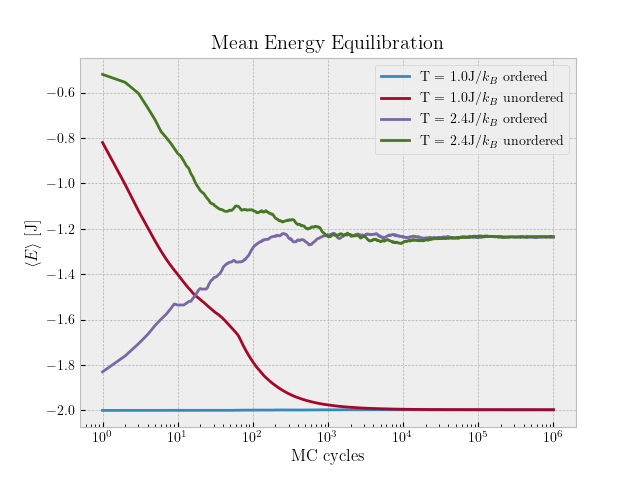
\includegraphics[width=0.95\linewidth]{./figures/Energy.png}
	\caption{The expectation values of the mean energy as a function of Monte Carlo cycles for a $20\times20$ lattice with two different initial spin configurations and two different temperatures. The ordered state refers to an initial spin configurations where all spins are pointing up. The unordered state is a random configuration. We see that the time for the system to reach the most likely state is around $10^4$ to $10^5$ cycles.}
	\label{fig:Energy}
\end{figure}
\begin{figure}
	\centering
	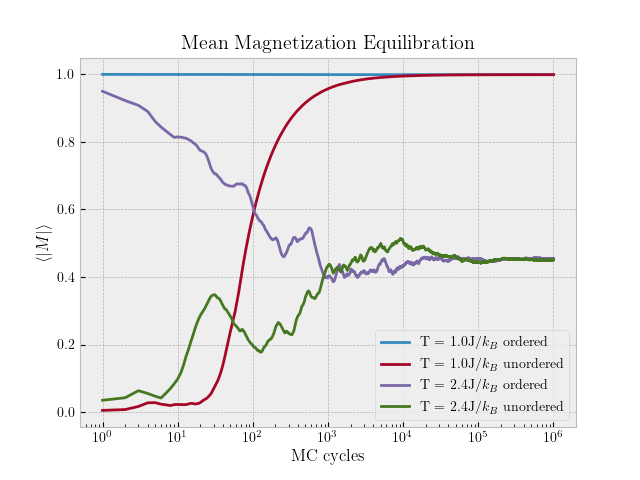
\includegraphics[width=0.95\linewidth]{./figures/Magnetization.png}
	\caption{The expectation values of the mean absolute magnetization as a function of Monte Carlo cycles for a $20\times20$ lattice with two different initial spin configurations and two different temperatures. The ordered state refers to an initial spin configurations where all spins are pointing up. The unordered state is a random configuration. We see that the time for the system to reach the most likely state is around $10^5$ cycles.}
	\label{fig:Magnetization}
\end{figure}
\subsection{Acceptance Ratio} %1
In figure \ref{fig:Accept} the number of accepted flips for different temperatures and initial configurations are plotted as a function of Monte Carlo cycles. Looking at $T=1.0$, we see that for the ordered initial configuration has close to a linear relation when the system starts to accept flips. For the unordered system we see that it follows a similar relation, but seems to reach equilibration a bit later. This can be read from figure \ref{fig:Energy} and figure \ref{fig:Magnetization}, which coincides with the points where the sharp edges in the lines between $10^1$ and $10^2$.

For the case for $T=2.4J/k_B$ we see that the unordered initial configuration almost instantly has a linear relation between accepted flips and Monte Carlo cycles. For the ordered start, it takes around $10^2$ cycles before it reaches a linear relation. 

What we can see applies regardless of initial configuration is the for a higher temperature, the system accepts more flips then for low temperatures. Which is supported by the Boltzmann distribution \eqref{eq:boltz}, where we get higher values for higher values of T.
\begin{figure}
	\centering
	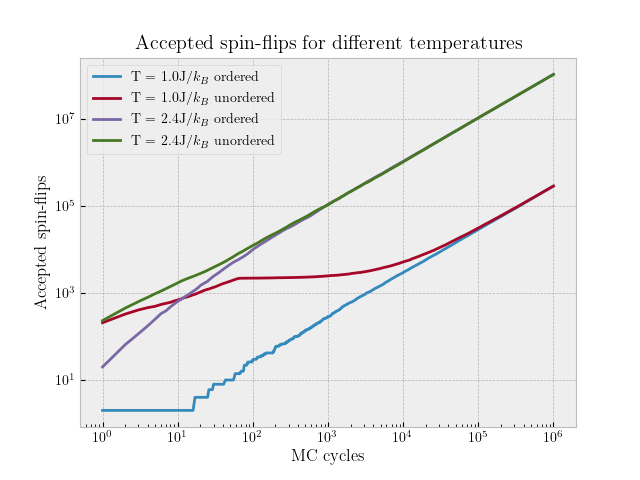
\includegraphics[width=0.95\linewidth]{./figures/Accept.png}
	\caption{Number of accepted flips as a function of Monte Carlo cycles for two different temperatures and two different initial spin configurations. The ordered state refers to an initial spin configurations where all spins are pointing up. The unordered state is a random configuration. All the lines trend to linear relations ships after around $10^5$ cycles, which is the same as equilibration time, for the systems shown in figure \ref{fig:Energy}.}
	\label{fig:Accept}
\end{figure}
\subsection{Probability Distribution} %1
Another interesting property to study is the probability distribution. In figure \ref{fig:ProbabilityDensity} we see the probability distribution for $T=1.0$ and $T=2.4$ for the system after it has reached the most likely state. The results are generated for a burn-in period of $10^5$ cycles and a total of $10^6$ samples. 

For $T=1.0$ we see that most of the energies are within one region, with a mean value of $\mu = -790.863[E/J]$. For $T=2.4$ we see a larger spread of values, similar to the Gaussian distribution, the mean value in this case it $\mu = -494.287[E/J]$.

In \autoref{tab:table1} the standard deviations of the energy $\sigma_E$, for both a unordered and ordered initial spin configuration.
\begin{figure*}
	\centering
	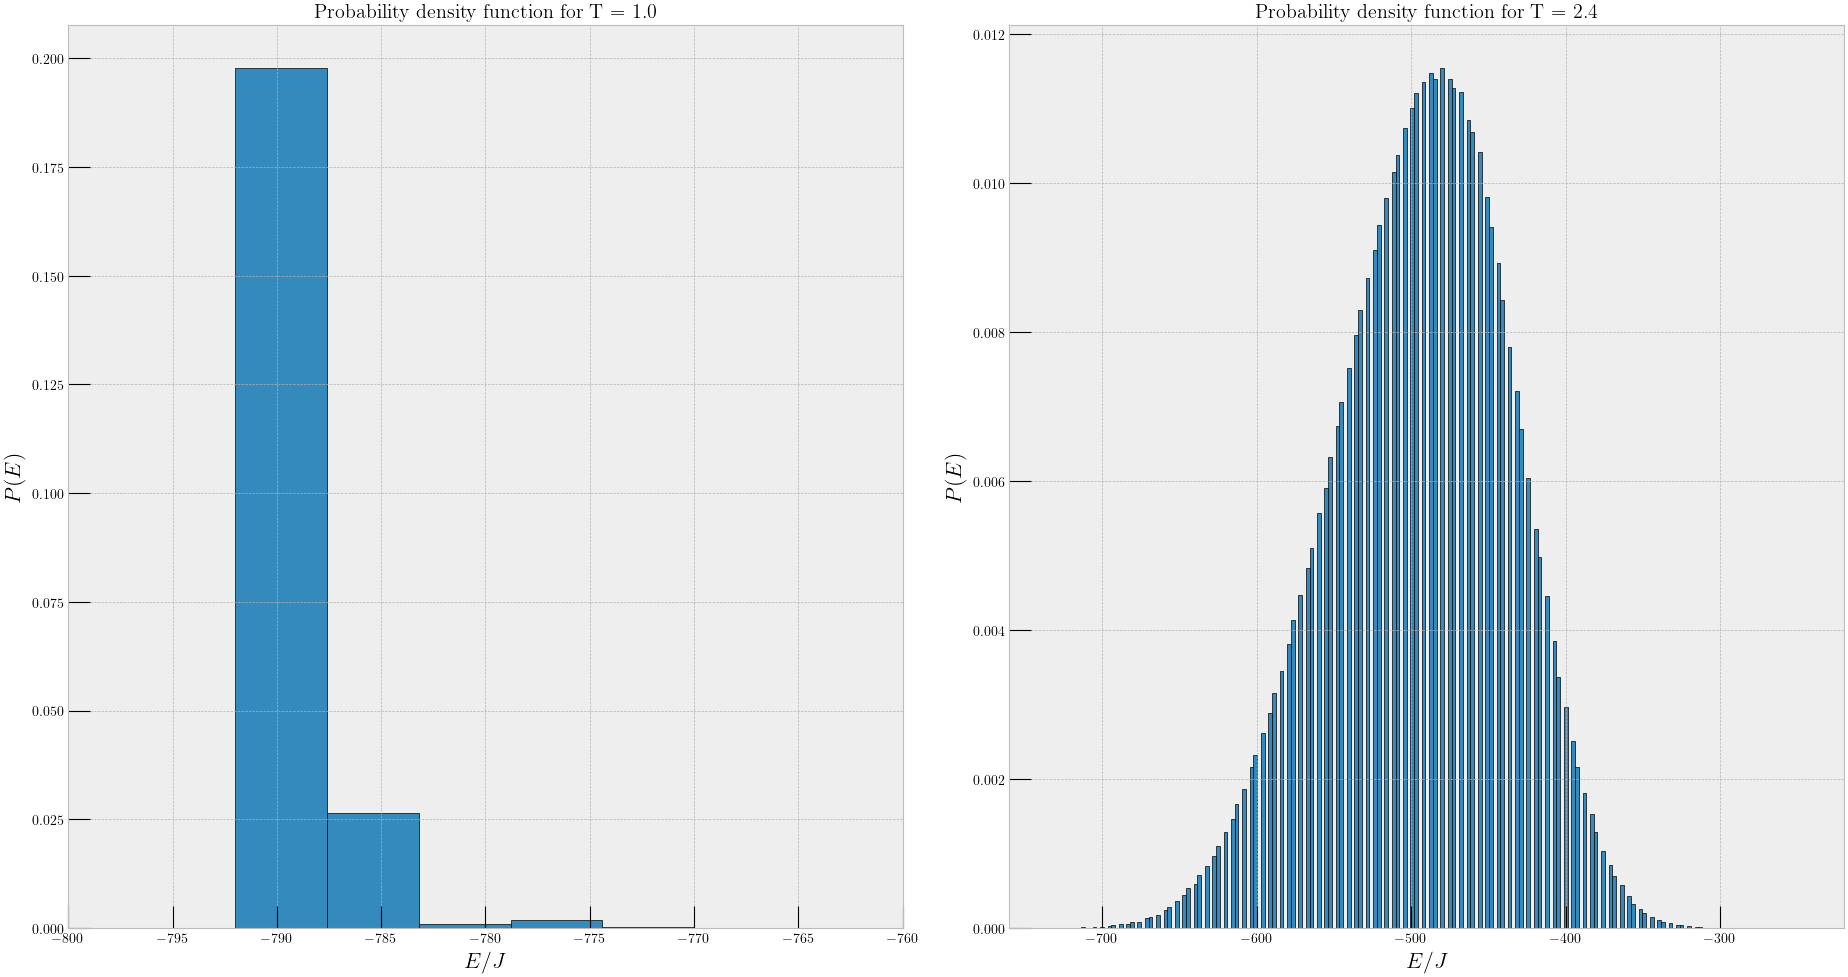
\includegraphics[scale=0.7]{./figures/ProbabilityDensity.png}
	\caption{Probability distribution of energy for temperatures $T=1.0$ and $T=2.4$, found by counting the number of appearances of an energy state. Calculations where done after most likely state has been reached.}
	\label{fig:ProbabilityDensity}
\end{figure*}

\begin{table}
	\centering
	\caption{The computed standard deviations of the energy $\sigma_E$ for both an ordered and a random starting spin configuration. The values where computed with a burn-in period of $\tau = 10^5$ and a total simulation time for t = $10^6$.}
	\label{tab:table1}
	\begin{tabular}{|c|c|c|}
		\hline
		$T$ & $\sigma_E$(Ground state initiation) & $\sigma_E$(Random initiation)\\
		\hline
		1.0 & 3.055921 &3.053113\\
		2.4 & 56.815100 &57.286746\\
		\hline
	\end{tabular}
\end{table}
\subsection{Parallelization and Optimization} %1
In figure \ref{fig:TimingRuns} we can see the gain for compiler flags and parallelization using MPI. The runs where done over different lattice size with $10^5$ Monte Carlo cycles. A wide range of compiler flags where tested, with both unparallelized and parallelized code to get a full picture. We can see that the runs with no compiler flags for the parallelized code performs only slightly worse than the unparallelized code with compiler flags. 
For the largest lattice size of $100\times 100$, the \texttt{-O3}, performs better than the rest. The parallelization runs where all done using 8 cores, of 1 GHz each, on an Intel i5 processor. 
\begin{figure}
	\centering
	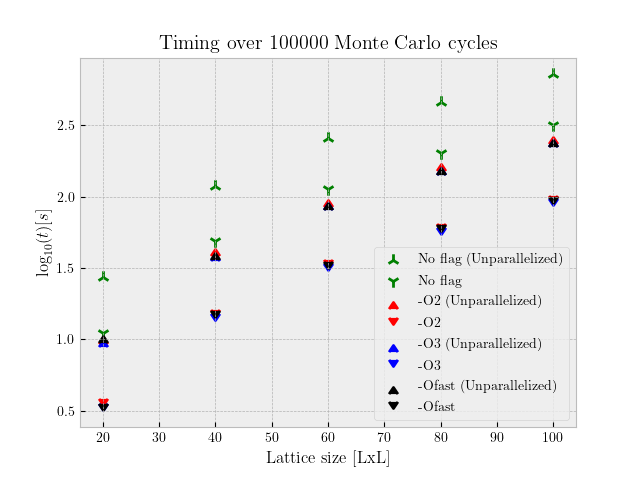
\includegraphics[width=0.95\linewidth]{./figures/TimingRuns.png}
	\caption{Timing runs, using a 8-core i5 Intel processor. Up arrows show the unparallelized runs, whilst down arrows display the parallelized runs. The data is displayed using a lograthmic scale along the y-axis to better display the difference between the runs.}
	\label{fig:TimingRuns}
\end{figure}
\subsection{Phase Transition} %1
The results displayed in figure \ref{fig:LatticeSize} where computed with varying temperature step and Monte Carlo cycles. In all cases $10\%$ of the total number of cycles where used as a burn-in period, before the system was sampled for the total number of cycles. A random initial state was used. 

For the $40\times 40$ lattice, a temperature step of $0.05$ was used, for the entire range of $T \in [2.0, 2.45]$. $6\cdot 10^6$ cycles where used. 
For the remaining lattice size a temperature step of $0.01$ has been used. Including the temperature range has been narrowed down to reduce computation time. 
The lattice size of $60\times 60$ and $80\times 80$, where found using $8\cdot 10^6$ cycles.
For the last size $100\times 100$, $1.6\cdot 10^7$ cycles where used. 

\begin{figure*}
	\centering
	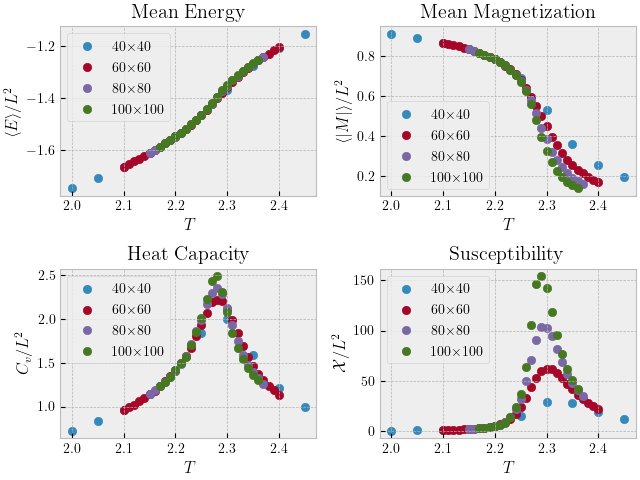
\includegraphics[scale=1]{./figures/LatticeSize.png}
	\caption{The data gathered from studying of the system of increasing lattice size. The data displayed is the mean energy, mean magnetization, specific heat and the susceptibility. A distinct peak is starting to form as we are increasing the lattice size in both susceptibility and specific heat. The mean magnetization also has a more distinct trend towards being divergent.}
	\label{fig:LatticeSize}
\end{figure*}

\subsection{Critical Temperature} %1
We used the specific heat to approximate the critical temperature, see figure \ref{fig:InterpolationCv}, by choosing the maximum values for the interpolation for different lattice sizes, to create a set of data points that we can study. The data points seen in figure \ref{fig:ApproxTc} are used to find the linear relation between the lattice size and critical temperature. The relation from equation \eqref{eq:3}, gives us that for a lattice of size $L = \infty$, the critical temperature is $T_c = 2.2665$. 
\begin{figure}
	\centering
	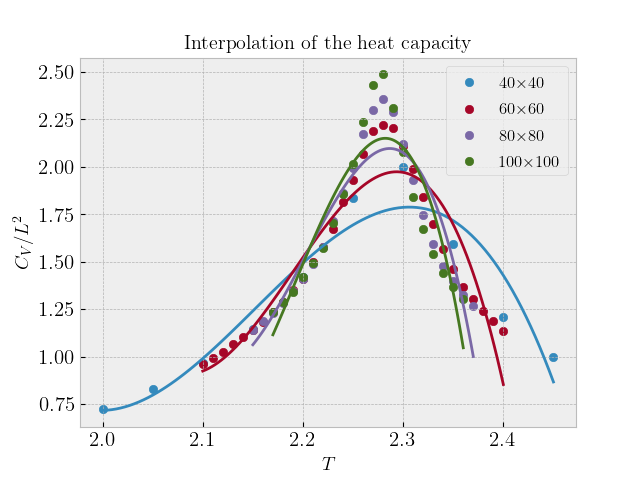
\includegraphics[width=0.95\linewidth]{./figures/InterpolationCv.png}
	\caption{Interpolation of the specific heat, 5-dimensional spline interpolation with smoothing. Low number of grid points lead to large discrepancy between the interpolation and the data points.}
	\label{fig:InterpolationCv}
\end{figure}
\begin{figure}
	\centering
	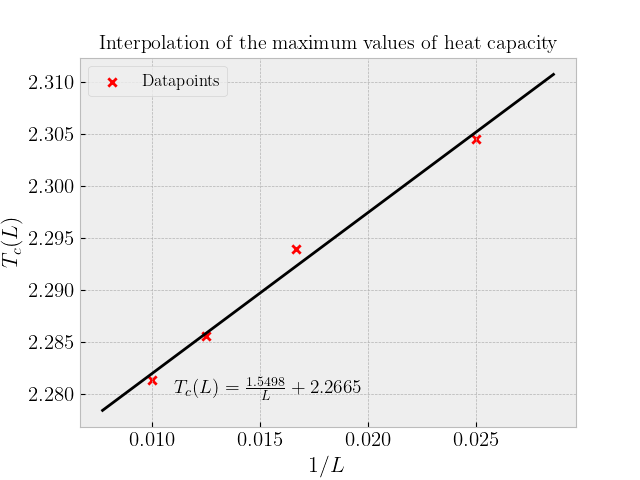
\includegraphics[width=0.95\linewidth]{./figures/ApproxTc.png}
	\caption{The max values of the interpolation in figure \ref{fig:InterpolationCv} has been used as data points. Linear regression of the data points gives the equation seen in the plot.}
	\label{fig:ApproxTc}
\end{figure}
\section{Discussion} %0
\subsection{Benchmark Test $2\times 2$ Lattice} %1
From \autoref{tab:tableordered} and \autoref{tab:tableunordered} we see that as the number of Monte Carlo cycles increase, the values converge towards the expectation values. This goes for both an unordered spin configuration and an ordered spin configuration. For a $2\times 2$ lattice, this has little impact on the values, as the configurations are fairly close to one another. 

We can conclude that our implementation of the Monte Carlo simulation, using Metropolis algorithm for deciding spins is correctly implemented. And we can start expanding to larger lattice sizes.

\subsection{Equilibration and Most Likely State} %1
For the $2\times 2$ lattice, we did not care about the system before we start to sample it. However this is essential when we want to sample a system using Monte Carlo methods. If we do not let the system reach its most likely state before we would need to perform a lot more Monte Carlo samples to reach our expectation values. To try to find the equilibration time, we look at it graphically as seen in figures \ref{fig:Energy} and \ref{fig:Magnetization}, from this we saw that for a total number of $10^6$ Monte Carlo cycles and different initial spin configurations, we need around $10^5$ cycles before we reach equilibrium. For $T=1.0$, this is more cycles than strictly necessary, however implementing a dynamic burn-in period is not a good choice. It would mean that we need to know details about the initial configuration and the current lattice size, which would be inefficient compared to having a general period for which one equilibrates the system. 

For $T=2.4$ we see that we would need around $10^5$ cycles before reaching equilibrium, which is $10\%$ of the total cycles used. This coincides with the general consensus of ignoring the first $10-15\%$ of the total cycles before starting ot sample the system. For this sampling, we are only studying the temperatures individually, so we are not concerned with how equilibration will affect the system when we let the system evolve. 

From figure \ref{fig:LatticeSize}, we see that the difference in sampled expectation values is large. When gathered the data we only equilibrated the system for the initial temperature. For the rest we assumed that the configuration of the lattice would be close to the most likely state for the next temperature. For our chosen temperature steps of $\Delta T = 0.01$ for the large lattice size, we still see that the difference in especially susceptibility and specific heat are large. This is to be expected due to the nature of the system we are studying, but looking at magnetization we see that around the critical temperature, the difference in the magnetization of the system is large. Whilst for the energy the values are all, seemingly evenly spaced. 

Based on this we can conclude and our belief in large numbers, we can conclude that using an initial burn-in period of $10\%$ of the total number of cycles, and reusing our lattice when increasing temperature is a good approach for reducing the total computational time. Also whilst data have large differences between different expectation values at different temperatures, from our trials for the $2\times 2$ lattice, we saw that as we collected more and more samples without a burn-in period, we still achieved close to the expectation values. So our choice of system evolution and burn-in period seems to be a valid choice for getting correct data.

For improvement and even smaller temperature step would be a better choice, however due to limitations in computational time, this was not achievable. This would have made the method even better and we could be sure that the system is in its most likely state just a few cycles into the new temperature. 

\subsection{Acceptance Ratio} %1
For the same $20\times 20$ system we used to approximate an equilibration time we looked at how many spin-flips where accepted by our system as a function of Monte Carlo cycles, this can be seen in figure \ref{fig:Accept}. 

From this we can see that for both temperatures the acceptance ration converges to a linear relation between accepts and Monte Carlo cycles. For both systems this happens somewhere around where they reach their most likely state. However for $T=2.4$ we see that both initial configurations that they reach a linear relation long before the proposed equilibration time of $10^5$ cycles.

This linear relationship for $T=2.4$, happens around $10^3$ cycles which is the same point where the systems are hovering around their most likely state. From this we can deduce that as the systems reach their most likely state, they will start to accept an equal amount of spin-flips each cycle. We can from the combination of the acceptance ration and studying how the mean magnetization and mean energy changes as a function of Monte Carlo cycles, a burn-in period, as stated earlier of around $10^5$. Where we could even start sampling both systems after $10^3$ cycles. This second fact supports our choice of system evolution, as we would only need around $10^3$ cycles to reach the most likely state from one system to another, or even less. 

Looking at how the acceptance ratio differs between $T=1.0$ and $T=2.4$, we see that for a higher temperature, the system accepts more spin-flips. From how our acceptance probability is defined, we know that the system accepts all flips to a lower energy, which for a higher temperature this range would be higher. If the max energy state is $E_9$ and that is the most likely state for our system, then all energy until $E_0$ would be accepted instantly. Secondly, for our system to not always reach the state of lowest energy, but its most likely state, we have a second condition for accepting the proposed flip. This is based on the Boltzmann distribution and change of energy, and for large temperatures the Boltzmann distribution returns larger values for the energy. As we are comparing a random number in the range $[0,1]$,  we would have a larger range of these numbers accepted when the temperature is higher. 
So the data we find is concurrent with our expectations of the system behavior. 

\subsection{Probability Distribution} %1
The probabilities seen in figure \ref{fig:ProbabilityDensity} were computed after steady state was reached, so the initial spin configuration should be irrelevant for the data. From \autoref{tab:table1} we see a small discrepancy in $\sigma_E$, which is attributed to a small sample size. However this is so small, it can come down to the behavior of random numbers. 

For the case of $T=1.0$ case, the probability of being in the ground state account for the majority of cases. Which is supported by the standard deviation, being small. Here the standard deviation is considered a quantitative measurement of the spread in the data set. Looking at the mean value for this case, we see it is at $-790E/J$ which is close to the ground state, with all spins pointing in one direction. This specific configuration should have a mean energy of $-800E/J$. 

As discussed previously the number of accessible energies increases with temperature which is reflected in the $T=2.4$ case. The probability distribution resembles that of a Gaussian distribution, with a mean value of $-494E/J$. We also see a large standard deviation, which is is concurrent with the large range of accessible energies. 
\subsection{Optimization} %1
The Monte Carlo methods are greedy, and the more samples you can get the better the method becomes for approximating different expectation values. This leads to great benefits from writing code which can be parallelized and vectorized. This will reduce the computational time needed for a large sample set. For our calculations we chose to have each core to run its own Monte Carlo simulation, meaning that for a 8 core system, we are able to perform 8 times the Monte Carlo cycles in the same time period. This is a great method for sampling the system many, many times at the cost of over all computational time. 

The other choice may have been to split up the total Monte Carlo cycles into smaller chunks and having each core run a small part of the total cycles. Or a combination of the two. 

From figure \ref{fig:TimingRuns} we see that the difference between a parallelized run with no flags and a unparallelized run with flags are close. This is done for 8 core runs, over a range of time values. Due to some unfortunate events, the runs using the parallelized code had a burn-in period enables, meaning the code did $10\%$ more cycles when running the timing runs. Regardless we see from the data how effective parallelization is on reducing run time, and would keep improving as we are able to add more and more core to the calculations by using larger computers and more processors. 

In turn we also see a large speedup using compiler flags where the $-O3$ flags shows the largest reduction in computational time. The flags $-O2$ and $-Ofast$ are close in performance, so any of the three can be used. 

\subsection{Phase Transition} %1
As our system increases in lattice size we expect the susceptibility and specific heat to diverge. For the mean magnetization we expect the system it should converge to with an infinite slope. The data from the study of phase transition can be seen in figure \ref{fig:LatticeSize}.

For the mean magnetization we see tendencies of this, as the slope gets gradually closer to the analytical critical temperature found by Lars Onsager, before flattening out. This supports our expected behavior of the mean magnetization. 

Regarding both the susceptibility and specific heat we are expecting to see increasing peaks getting closer to the critical temperature from above. This behavior is represented in figure \ref{fig:LatticeSize}, where the peaks move to the left as expected. We also see increasing peaks, which gets a sharper edge. 

What would have been preferred would be a smaller temperature step, leading to more grid points and a clearer representation of behavior. This was limited by the computational time needed for the implemented methods of parallelization and the limit in available computational time. 
\subsection{Critical Temperature} %1
Lastly we looked at approximating the critical temperature found by Lars Onsager, using the linear relation between lattice size and critical temperature. 
The method used to do this, is studying the specific heat and using 5-dimensional spline method to and extracting the maximum values of the interpolation, see figure \ref{fig:InterpolationCv}. These maximas are used as the set of data points to approximate the linear relation in equation \eqref{eq:3}, the result of this can be seen in figure \ref{fig:ApproxTc}. 

From this can extract that the critical temperature at $L=\infty$ is $T_c = 2.2665$. This is lower than the critical temperature found by Lars Onsager. Important fact about our method for finding the critical temperature, is that we are using a double interpolation, and in computing our estimate of the critical temperature we do not account for the error in the spline interpolation. Our estimate of the critical temperature in the thermodynamic limit, $L=\infty$, can only be taken as preliminary. Our results only confirms that there exists a phase transition in the thermodynamic limit. 

The results could have been found by using both the specific heat and the susceptibility, in addition to having more data points to interpolate. This would lead to a better estimate of the interpolation curves with a smaller deviation, our data set suffers from a lack of mesh points and a large deviation between the interpolation and the found expectation values. 

\section{Conclusion} %0
In this article we have studied the 2-dimensional Ising model with the purpose of confirming physical properties of ferromagnetic materials, with the use of Monte Carlo methods with Metropolis sampling. 
We started off by studying a $2\times 2$ lattice, before expanding and improving our code to be able to studying large lattice size with ease. A lattice size of around $10^6$ was required to get close to the analytical results for the $2\times 2$ lattice. From a $20\times 20$ lattice we looked at how the equilibration time behaves for different temperatures and how this can be chosen. We found that a burn-in period of around $10^5$ cycles or $10\%$ of the total cycles, this coincides with the acceptance ratio we found. 
Further we studied the probability distribution, this is numerically impossible to calculate for larger lattice sizes, but by sampling the system after it has reached its most likely state, we can get a good idea of how it looks. By taking enough samples we can find a very good approximation of the function, as the accuracy of Monte Carlo simulations is dependent directly on the number of samples. 

To be able to study larger systems, we needed to improve our code base to be able to handle the lattice sizes. This was done by parallelization and compiler flags which showed a significant reduction in run time, in both cases. So a combination of the two was utilized to satisfy the greedy Monte Carlo simulations. 
With this optimization we looked to expand our lattice, to study phase transition, this is an expected physical property of the Ising model. As we expanded our lattice we found that the system behaves as expected and we can draw conclusion that it is converging towards the physical system we are trying to replicate. 

The last property we looked at is the critical temperature found by Lars Onsager\cite{LarsOnsager} to be $T_c = 2.269...$, in 1944. For our simulations we found by interpolation that the critical temperature is $\tilde{T}_c = 2.266$, which can only be taken as a preliminary result as our approximation is based on a double interpolation, with no regards to the error of either interpolation. 
\bibliography{bib_proj4}
\bibliographystyle{plain}


\end{document}
